\documentclass[11pt,a4paper,openany]{book}
\usepackage{ctex}
\usepackage{fontenc,xunicode,xltxtra}
\usepackage{changepage}
\usepackage{amsmath,amsthm}
\usepackage{amssymb}
\usepackage{lmodern}
\usepackage{graphicx}
\usepackage{epstopdf}
\usepackage{enumerate}
\usepackage[english]{babel}
\usepackage{amsmath}
\usepackage{amssymb}
\usepackage{latexsym}
\usepackage{multirow}
\usepackage{bigdelim}
\usepackage{color}
\usepackage{graphicx}
\usepackage{wrapfig}
\usepackage{picinpar}
\usepackage{picins}
\usepackage{float}
\usepackage{clrscode}
\usepackage{algorithm} %format of the algorithm
\usepackage{algorithmic} %format of the algorithm
\usepackage{subfigure}
\usepackage{xeCJK}
\usepackage{varwidth}
\usepackage{caption}
\usepackage{lipsum}
\usepackage{framed}
\usepackage[colorlinks]{hyperref}

\setCJKmainfont[BoldFont=SimHei,ItalicFont=KaiTi]{宋体}
\setmonofont{宋体}    % 等寬字型
\setmainfont{Times New Roman}  %缺省英文字体

\XeTeXlinebreaklocale "zh"   % 针对中文进行断行
\XeTeXlinebreakskip = 0pt plus 1pt minus 0.1pt     % 给予TeX断行一定自由度
%\linespread{1.5}                                  % 1.5倍行距

\newfontfamily{\H}{SimHei}
\newfontfamily{\K}{KaiTi}
\newfontfamily{\S}{黑体}
\setCJKfamilyfont{hwxw}{STXinwei}                    %华文新魏  hwxw
\newcommand{\hwxw}{\CJKfamily{hwxw}}
\setCJKfamilyfont{hei}{SimHei}                       %黑体  hei
\newcommand{\hei}{\CJKfamily{hei}}
\setCJKfamilyfont{song}{SimSun}                      %宋体 song
\newcommand{\song}{\CJKfamily{song}}
\setCJKfamilyfont{kai}{KaiTi}                        %楷体  kai
\newcommand{\kai}{\CJKfamily{kai}}
\setCJKfamilyfont{fs}{FangSong}                      %仿宋 fsong
\newcommand{\fs}{\CJKfamily{fs}}

\newcommand{\xiaosihao}{\fontsize{12pt}{\baselineskip}\selectfont}  %字体大小
\newcommand{\wuhao}{\fontsize{10.5pt}{\baselineskip}\selectfont}

\captionsetup[figure]{name=图}
\captionsetup[table]{name=表}
\definecolor{shadecolor}{rgb}{0.92,0.92,0.92}

%\makeatletter
%\makeatother
\newtheorem{theorem}{\textbf{定理}}[section]
\newtheorem{defination}{\textbf{定义}}[section]
\newtheorem{property}{\textbf{性质}}[section]
\newtheorem{lemma}{\textbf{引理}}[section]
\newtheorem{coro}{\textbf{推论}}[section]
\newtheorem{sample}{\textbf{例}}[section]
\newtheorem{guess}{\textbf{猜想}}[section]
\renewcommand{\figurename}{图}
\floatname{algorithm}{算法}
\newcommand{\reffig}[1]{\textcolor{red}{图}\ref{#1}}

\usepackage{fancyhdr}
%\fancyhf{}
\fancyhead[LO,RE]{\leftmark}
\fancyhead[LE,RO]{cumtb.iis.ddb}
\fancyfoot[LO,RE]{}
\fancyfoot[LE,RO]{-\,\thepage\,-}
\renewcommand{\headrulewidth}{0pt}

\fancypagestyle{plain}{
     \fancyhf{}
     \fancyfoot[LO,RE]{}
     \fancyfoot[LE,RO]{-\,\thepage\,-}
     \renewcommand{\headrulewidth}{0pt}
}

\usepackage{titlesec}
\titleformat{\chapter}{\centering\huge\hei}{第\,\thechapter\,章}{1em}{}[\vspace{-1cm}]
\begin{document}
\pagestyle{plain}  %取消页码
\chapter{基本概念}
\section{图论概述}
\paragraph{}\textbf{离散数学}是以研究离散量的结构和相互之间的关系为主要目标,其研究对象一般是有限个或可数个元素。离散数学充分契合了计算机科学的特点。离散数学是计算机科学重要的基础理论之一。\\
离散数学主要包括四个方面:数理逻辑、集合论、图论、代数机构。\\
\paragraph{}\textbf{图论[Graph Theory]}是数学的一个分支,它以图为研究对象。\\
\indent 世界上各事物之间,自然界内诸现象之间经常存在着某些必然的联系,需要人们通过研究分析,去揭示这些关系。\\
\indent 人们常把事物、现象用\textcolor[rgb]{1.00,0.00,0.00}{结点}表示,用有向或无向的\textcolor[rgb]{1.00,0.00,0.00}{边}来表示它们之间的联系。这就构成了图论中所讨论的\textcolor[rgb]{1.00,0.00,0.00}{图}。\\
\indent 历史上图论曾经被好多位数学家各自独立地建立过。关于图论的文字记载最早出现在欧拉1736年论著中,其原始问题有很强的实际背景。18世纪在哥尼斯堡城(今俄罗斯加里宁格勒)的普莱格尔河上有7座桥\footnote{在第二章欧拉回路中介绍},将河中的岛屿和河岸连结。\\
\begin{figure}[H]
  \centering
 % \vspace{-10pt}
  \begin{minipage}[!ht]{.35\linewidth}
  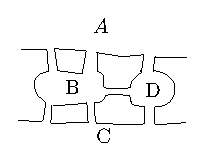
\includegraphics[width=1.0\linewidth]{2_8.eps}
  \caption{哥尼斯堡7桥}
  \end{minipage}
  \begin{minipage}[!ht]{.35\linewidth}
   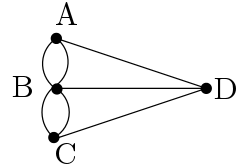
\includegraphics[width=1.0\linewidth]{2.9.png}
  \caption{哥尼斯堡7桥简化}
  \end{minipage}
  %\vspace{0pt}
\end{figure}
\kai{早期的图论与数学游戏有密切的联系:周游世界问题、渡河问题、三家三井问题...20世纪后,图论的应用渗透到其它学科领域,如物理、化学、运筹学、博弈论、计算机网络、社会学、语言学等等。对于基础图论来说,不要求事先掌握高深的数学工具,只需要有集合论和线性代数的基本概念,即可进行学习。}\\

\section{图的基本概念及定义}
\begin{defination}
二元组$G=(V(G),E(G))$称为图。其中$V(G)$是非空集,称为结点集;$E(G)$为$V(G)$各结点之间边的集合,称为边集。\\
\end{defination}
\noindent 常用$G=(V,E)$表示图。\\
当V,E都是有限集合时,称G为\textcolor[rgb]{1.00,0.00,0.00}{有限图}。\\
当V或E是无限集合时,称G为\textcolor[rgb]{1.00,0.00,0.00}{无限图}。\\
一般情况下,给定$G=(V,E)$,如不加特殊说明,认为$V=\{v_1,v_2,v_3,\cdots,v_n\}$,$E=\{e_1,e_2,e_3,\cdots,e_m\}$,即结点数$|V|=n$,边数$|E|=m$。\\
\\
若图中的边为有向的,则称为有向图。\\
若图中的边为无向的,则称为无向图。\\
若图中既有有向边,又有无向边,则称为混合图。\\
\begin{figure}[H]
  \centering
  % Requires \usepackage{graphicx}
  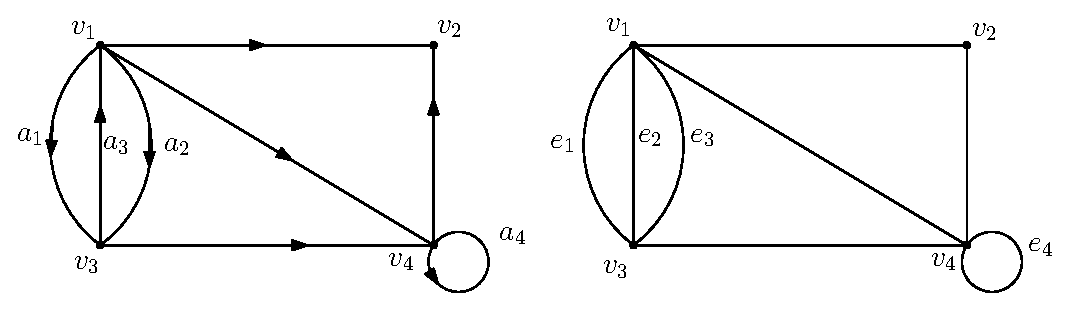
\includegraphics[width=0.9\textwidth]{1_3.eps}\\
  \caption{}
\end{figure}
\noindent 图的边可用$e_k=(v_i,v_j)$表示\\
\vspace{-20pt}
\begin{enumerate}
  \item 称$v_i$与$v_j$是\textcolor[rgb]{1.00,0.00,0.00}{相邻结点}
  \item 称$e_k$分别与$v_i,v_j$\textcolor[rgb]{1.00,0.00,0.00}{相关联}
  \item 如果$e_k$是有向边,称$v_i$是$e_k$的\textcolor[rgb]{1.00,0.00,0.00}{始点},$v_j$是$e_k$的\textcolor[rgb]{1.00,0.00,0.00}{终点},
  并称为$v_i$是$v_j$ 的\textcolor[rgb]{1.00,0.00,0.00}{直接前驱},$v_j$是$v_i$的\textcolor[rgb]{1.00,0.00,0.00}{直接后继}
  \item 如果$e_k$是无向边,称$v_i,v_j$是$e_k$的两个\textcolor[rgb]{1.00,0.00,0.00}{端点}
\end{enumerate}
\begin{defination}
只与一个结点相关联的边称为\textcolor[rgb]{1.00,0.00,0.00}{自环};在同一对结点之间可以存在多条边,称为\textcolor[rgb]{1.00,0.00,0.00}{重边};
含有重边的图叫\textcolor[rgb]{1.00,0.00,0.00}{多重图}。
\end{defination}
\begin{defination}
$G=(V,E)$的某结点所关联的边数称为该结点的度,用$d(v)$表示。如果$V$带有自环,则自环对$d(v)$的贡献为2。\\
有向图中:
\vspace{-15pt}
\begin{itemize}
  \item[-] 以结点V为始点的边数目称为V的正度,记为$d^{+}(v)$
  \item[-] 以结点V为终点的边数目称为V的负度,记为$d^{-}(v)$
\end{itemize}
显然,有$d^{+}(v)+d^{-}(v)=d(v)$
\end{defination}
\begin{defination}
任意两结点间最多只有一条边,且不存在自环的无向图称为\textcolor[rgb]{1.00,0.00,0.00}{简单图}。\\
没有任何边的简单图叫\textcolor[rgb]{1.00,0.00,0.00}{空图},记为$N_n$。\\
任何两结点间都有边的简单图称为\textcolor[rgb]{1.00,0.00,0.00}{完全图}记为$K_n$。($K_n$中每个结点的度为n-1)
\end{defination}
\begin{property}
{设$G=(V,E)$有n个结点,m条边,则}$$\sum_{v\in V(G)}(d_v)=2m$$
\end{property}

\begin{property}
G中度为奇数的结点必为偶数个。
\end{property}
\begin{property}
有向图G中正度之和等于负度之和。
\end{property}
\begin{property}
$K_n$中的边数为$\frac{1}{2}n(n-1)$。
\end{property}
\begin{property}
非空简单图中一定存在度相同的结点。
\end{property}

\begin{defination}
如果图$G=(V,E)$的每条边$e_k=(v_i,v_j)$都赋予一个实数$W_k$做为该边的\textcolor[rgb]{1.00,0.00,0.00}{权},则称G为\textcolor[rgb]{1.00,0.00,0.00}{赋权图}。
如果这些权都是正实数,就称G为\textcolor[rgb]{1.00,0.00,0.00}{正权图}。
\begin{figure}[H]
  \centering
  % Requires \usepackage{graphicx}
  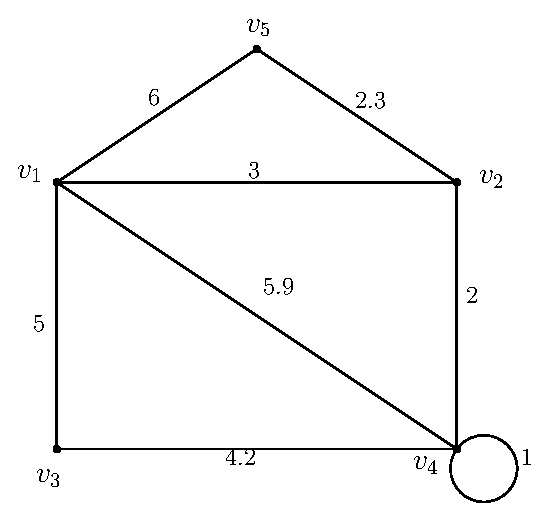
\includegraphics[width=0.5\textwidth]{1_4.eps}\\
  \caption{}
\end{figure}

\end{defination}

\begin{defination}
给定$G=(V,E)$,如果存在另一个图$G'=(V',E')$,满足$V'$包含于V,满足$E'$包含于E,则称$G'$是G的一个\textcolor[rgb]{1.00,0.00,0.00}{子图}。\\
如果$V'=V$,就称$G'$是G的\textcolor[rgb]{1.00,0.00,0.00}{支撑子图}。\\
如果$V'$包含于V,且$E'$包含了在结点子集$V'$之间的所有边,则称$G'$是G的\textcolor[rgb]{1.00,0.00,0.00}{导出子图}。\\
\begin{figure}[H]
  \centering
  % Requires \usepackage{graphicx}
  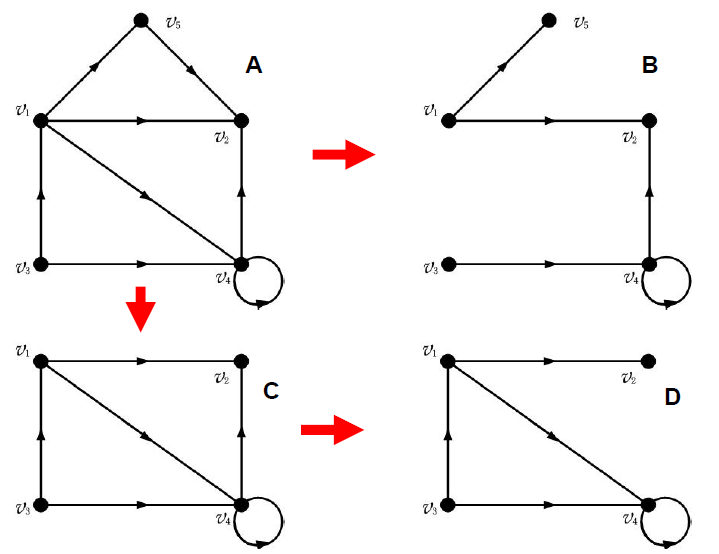
\includegraphics[width=0.8\textwidth]{1.5.png}\\
  \caption{B:支撑子图 C:导出子图 D:子图}
\end{figure}
\end{defination}
\begin{coro}
显然,根据上述的定义,图G是自身的子图,支撑子图,导出子图。\\
\\
空图是图G的支撑子图。\\
\end{coro}
\begin{defination}
称原图G和空图都是图G的\textcolor[rgb]{1.00,0.00,0.00}{平凡子图}。\\
\end{defination}
\begin{defination}
给定两个图$G_1=(V_1,E_1),G_2=(V_2,E_2)$。令
\begin{gather}
  G_1\bigcup G_2=(V_1\bigcup V_2,E_1\bigcup E_2) \\
  G_1\bigcap G_2=(V_1\bigcap V_2,E_1\bigcap E_2)\\
  G_1\bigoplus G_2=(V_1\bigoplus V_2,E_1\bigoplus E_2)
\end{gather}
$1.1,1.2,1.3 $分别称为$G_1$和$G_2$的\textcolor[rgb]{1.00,0.00,0.00}{并}、\textcolor[rgb]{1.00,0.00,0.00}{交}、\textcolor[rgb]{1.00,0.00,0.00}{对称差}。\\
\begin{figure}[H]
  \centering
  % Requires \usepackage{graphicx}
  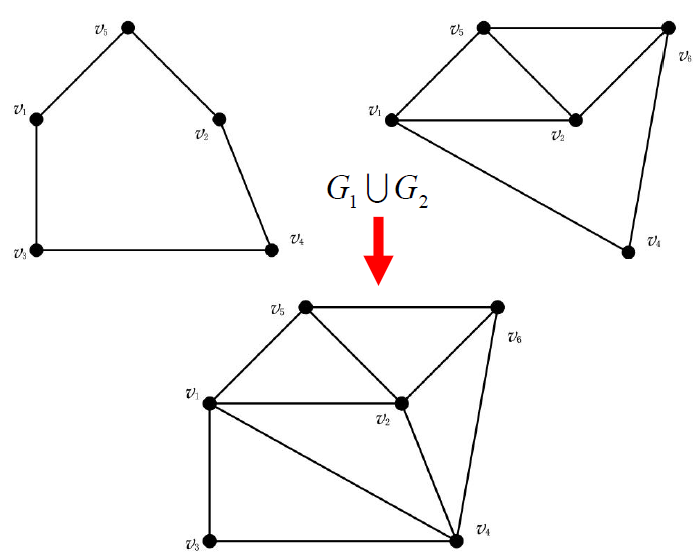
\includegraphics[width=0.8\textwidth]{1.6.1.png}\\
  \caption{$G_1\bigcup G_2$}
\end{figure}
\begin{figure}[H]
  \centering
  % Requires \usepackage{graphicx}
  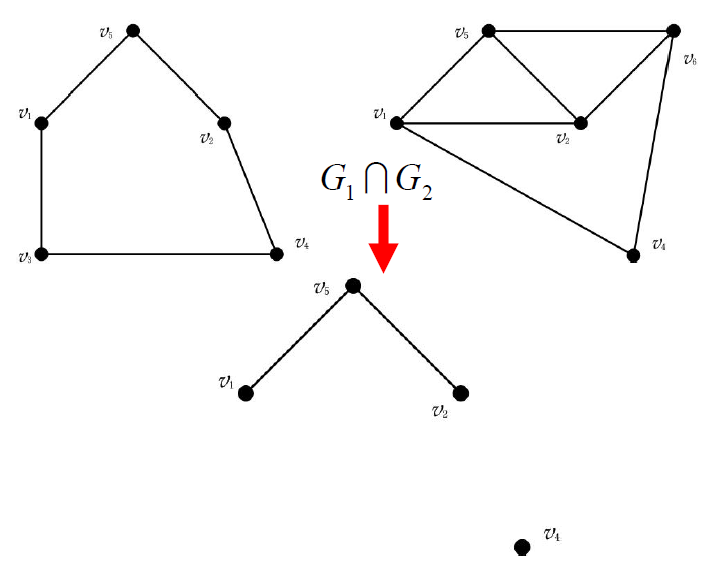
\includegraphics[width=0.8\textwidth]{1.6.2.png}\\
  \caption{$G_1\bigcap G_2$}
\end{figure}
\begin{figure}[H]
  \centering
  % Requires \usepackage{graphicx}
  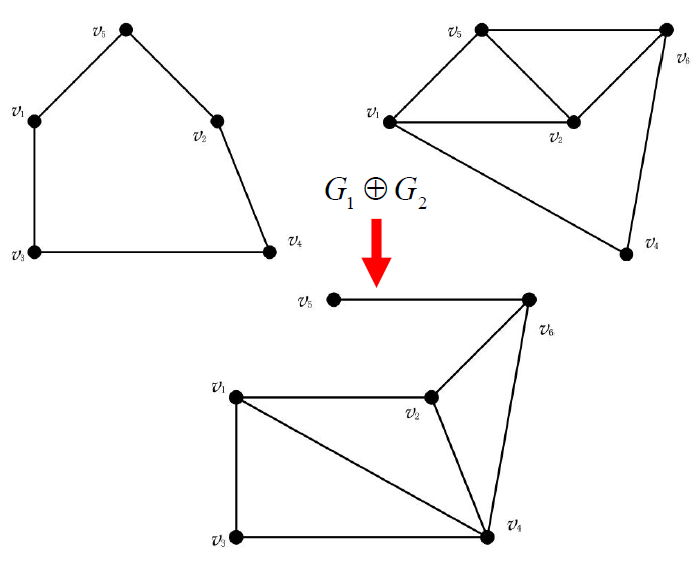
\includegraphics[width=0.8\textwidth]{1.6.3.png}\\
  \caption{$G_1\bigoplus G_2$}\label{fig:163}
\end{figure}
\end{defination}
\song
{
在图G中删掉一个子图H,指删掉H中的各条边,记为\textcolor[rgb]{1.00,0.00,0.00}{$G\quad -\quad H$}。\\
对于简单图G,称$K_n - G$为G的\textcolor[rgb]{1.00,0.00,0.00}{补图},记做\textcolor[rgb]{1.00,0.00,0.00}{$\bar{G}$}。\\
从G中删去某个结点$v$及其关联的边所得到的图记做\textcolor[rgb]{1.00,0.00,0.00}{$G-v$}。\\
从G中删掉某条特定的边e,记做\textcolor[rgb]{1.00,0.00,0.00}{$G-e$}。\\
显然,$G-v$是图G的导出子图,$G-e$是图G的支撑子图。\\
}
\begin{defination}
如G为无向图,则$$\Gamma(v)=\{u|(v,u)\in E\}$$称为v的\textcolor[rgb]{1.00,0.00,0.00}{邻点集}。\\
如G为有向图,v是其中一个结点,则$$\Gamma^{+}(v)=\{u|(v,u)\in E\}$$称为v的直接后继或者\textcolor[rgb]{1.00,0.00,0.00}{外邻集};相应的
$$\Gamma^{-}(v)=\{u|(v,u)\in E\}$$称为v的直接前趋集或内邻集。\\
\end{defination}

\begin{defination}
两个图$G_1=(V_1,E_1),G_2=(V_2,E_2)$,如果$V_1$,$V_2$之间存在双射$f$,而且$(u,v)\in E_1$,当且仅当$(f(u),f(v))\in E_2$时,称$G_1$和$G_2$\textcolor[rgb]{1.00,0.00,0.00}{同构}。记做$$G_1\cong G_2$$\\
\end{defination}
\begin{shaded}
\noindent 从定义知,若$G_1\cong G_2$,必须满足:\\
(1)$|V(G_1)|=|V(G_2)|$,$|E(G_1)|=|E(G_2)|$\\
(2)$G_1$和$G_2$结点度的非增序列相同\\
(3)$G_1$和$G_2$存在同构的导出子图\\
\end{shaded}
{\xiaosihao\hwxw 思考:如何判定两图同构?}\\
\begin{figure}[H]
  \centering
  % Requires \usepackage{graphicx}
  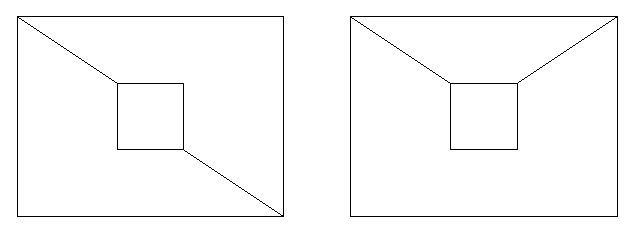
\includegraphics[width=0.8\textwidth]{tonggou.eps}\\
  \caption*{}
\end{figure}
\section{图的代数表示}
图在计算机中如何表示(拓扑结构、边权值...)?如何对图进行描述或运算?所以我们需要用代数的方法来描述图!\\
\begin{defination}
表示了结点间的邻接关系的矩阵称为\textcolor{red}{邻接矩阵}。\\
\end{defination}
\begin{shaded}
\noindent 有向图的邻接矩阵$\mathbf{A}$是一个n 阶方针,其元素为:
$$\mathbf{A}=[a_{ij}]_{n\times n} \quad a_{ij}=\begin{cases}
        1& (v_i,v_j)\in E\\
        0& others
    \end{cases}$$
\end{shaded}
\begin{figure}[H]
  \centering
  % Requires \usepackage{graphicx}
  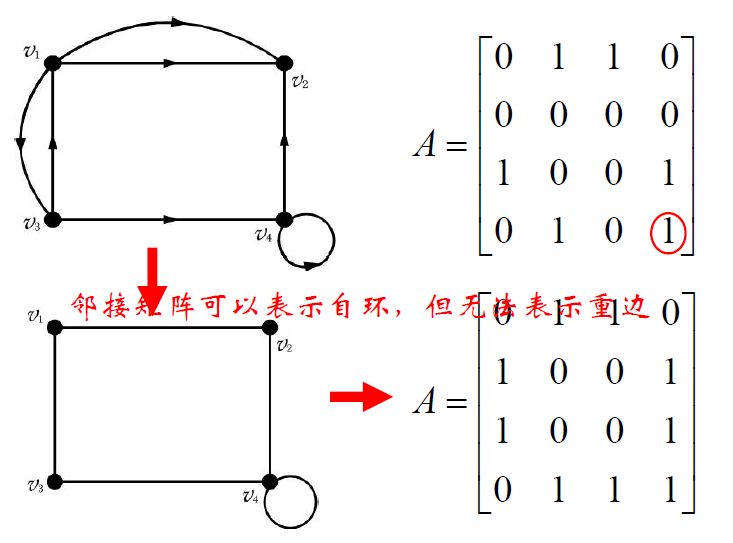
\includegraphics[width=0.8\textwidth]{1.9.png}\\
  \caption{}
\end{figure}
\textcolor{red}{权矩阵:}赋权图常用权矩阵A进行表示。
\begin{shaded}
其元素为:
$$\mathbf{A}=[a_{ij}]_{n\times n} \quad a_{ij}=\begin{cases}
        w_{ij}& (v_i,v_j)\in E\\
        0& others
    \end{cases}$$
\end{shaded}
\begin{figure}[H]
  \centering
  % Requires \usepackage{graphicx}
  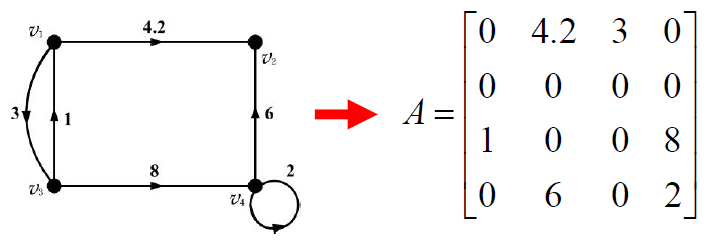
\includegraphics[width=0.8\textwidth]{1.10.png}\\
  \caption{}
\end{figure}
\textcolor{red}{关联矩阵:}关联矩阵表示结点与边之间的关联关系。\\
\begin{shaded}
有向图G的关联矩阵$\mathbf{B}$是$n\times m$的矩阵,当给定结点和边的编号之后,其元素
$$\mathbf{B}=[b_{ij}]_{n \times m} \quad b_{ij}=
\begin{cases}
        1& e_j=(v_i,v_k)\in E\\
        -1& e_j=(v_k,v_i)\in E\\
        0& others
    \end{cases}
$$
\end{shaded}
\begin{figure}[H]
  \centering
  % Requires \usepackage{graphicx}
  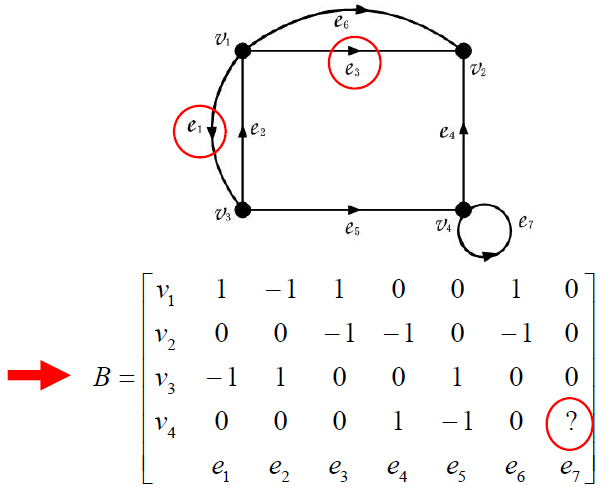
\includegraphics[width=0.8\textwidth]{1.11.png}\\
  \caption{}
\end{figure}
\begin{shaded}
无向图G的关联矩阵$\mathbf{B}$是$n\times m$的矩阵,当给定结点和边的编号之后,其元素
$$\mathbf{B}=[b_{ij}]_{n \times m} \quad b_{ij}=
\begin{cases}
        1& e_j \text{与}v_i\text{关联}\\
        0& others
    \end{cases}
$$
\end{shaded}
\begin{figure}[H]
  \centering
  % Requires \usepackage{graphicx}
  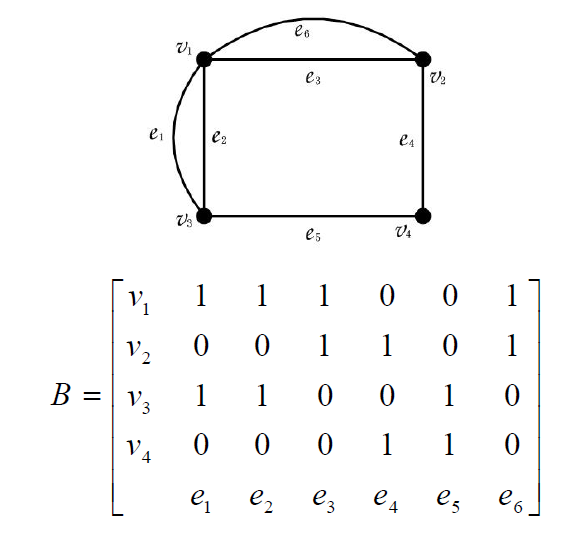
\includegraphics[width=0.8\textwidth]{1.12.png}\\
  \caption{}
\end{figure}
\begin{shaded}
\noindent 关联矩阵的性质(有向图):\\
(1)每列只有两个非零元:1、-1\\
(2)第$i$行非零元的数目恰为结点$v_i$的度,其中1的数目为其正度,-1的数目为其负度\\
关联矩阵的性质(无向图):\\
(1)每列只有一个非零元:1\\
(2)第i行1的数目恰为结点$v_i$的度\\
\textbf{关联矩阵能够表示重边,但不能表示自环。}
\end{shaded}

\textcolor{red}{邻接矩阵、权矩阵、关联矩阵可以表示重边,但无法表示自环}\\
邻接矩阵、权矩阵、关联矩阵的优点是一旦写出代数表达式,则可得到确定图,且非常直观。缺点是(1)不能表示自环(2)在计算机上存储邻接矩阵与关联矩阵时,将占据较大的存储空间并可能增加计算复杂度。所以需要引入\textbf{边列表}、\textbf{正向表}、\textbf{逆向表}、\textbf{邻接表}。\\

\end{document}
